\chapter{Конструкторская часть}

\section{Требования к программному обеспечению}

К разрабатываемой программе предъявлен ряд требований:

\textbf{Входные данные:} Взвешенный неориентированный граф, заданный матрицей стоимостей.

\textbf{Выходные данные:} Оптимальный гамильтонов цикл, в случае метода полного перебора, субоптимальный гамильтонов цикл в случае муравьиного алгоритма.

\section{Алгоритм полного перебора}

\subsection{Метод генерации перестановок}

Основной частью алгоритма полного перебора является алгоритм генерации перестановок, так как гамильтонов путь, как и гамильтонов путь, являются перестановками множества узлов графа. Существуют множество методов генерации перестановок~\cite{perms} как рекурсивных, так и итеративных. 
В данной работе будет использоваться нерекурсивный метод Хипа (Heap's method) разработанный в~\cite{perms-methods}.

\subsection{Алгоритм}

На рисунке~\ref{fig:permutations} представлен алгоритм полного перебора для решения задачи коммивояжёра.

\begin{figure}[h]
	\centering
	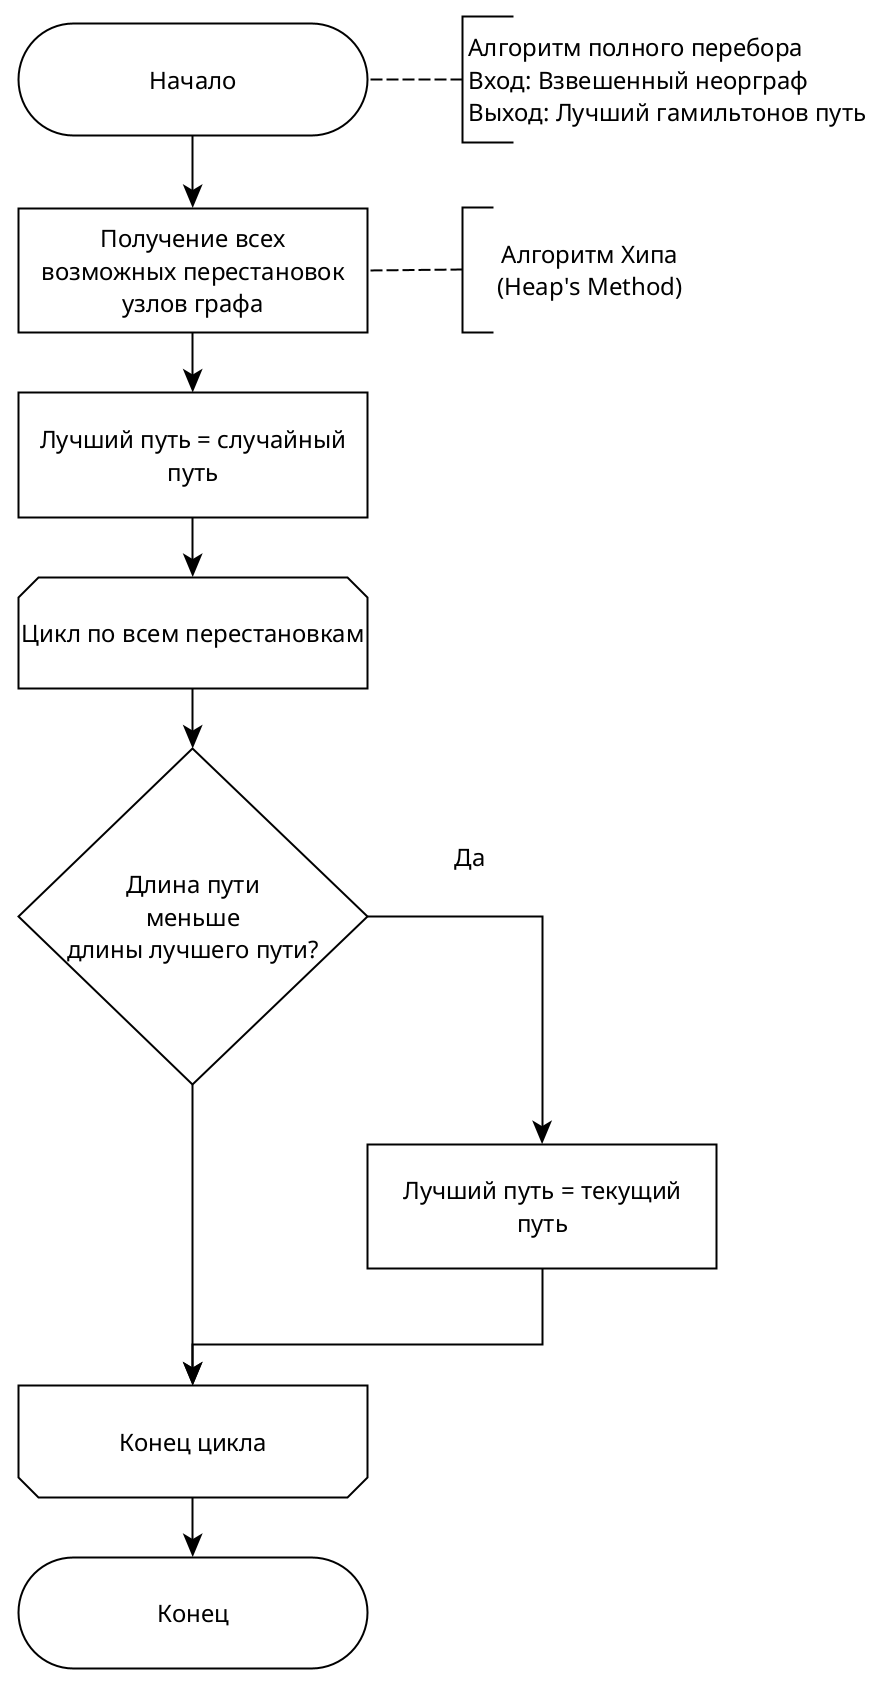
\includegraphics[width=0.5\textwidth]{permutations}
	\caption{Схема алгоритма полного перебора}
	\label{fig:permutations}
\end{figure}

\clearpage

\section{Муравьиный алгоритм}

На рисунках~\ref{fig:ant1} и~\ref{fig:ant2} представлен алгоритм муравьиного алгоритма для неорграфа с элитными муравьями.

\begin{figure}[h]
	\centering
	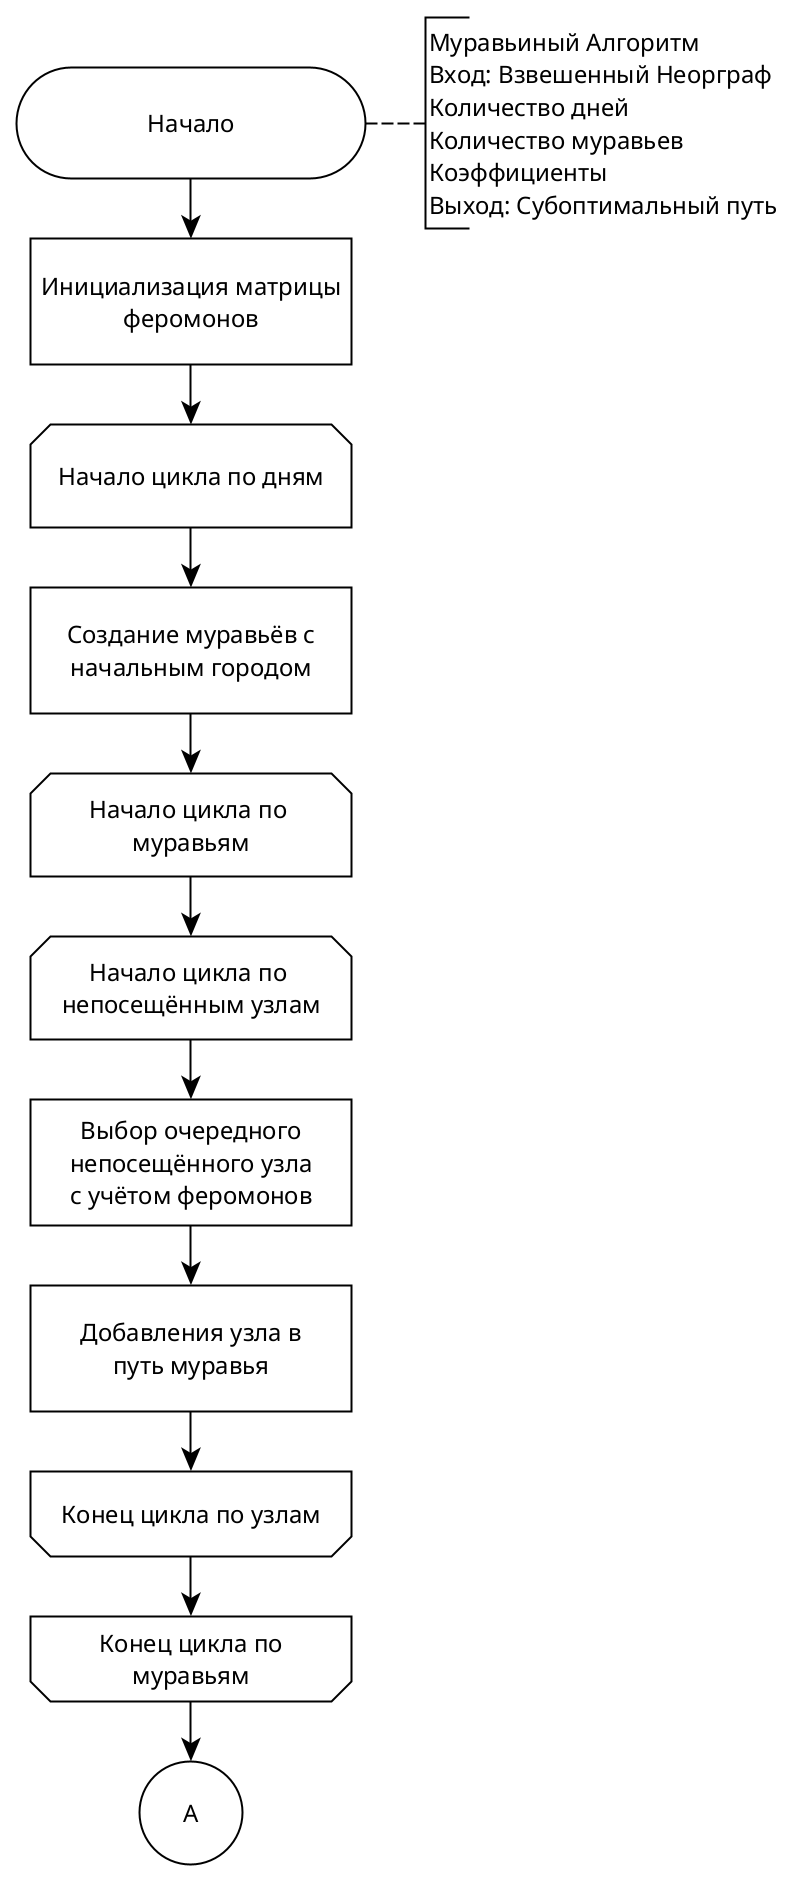
\includegraphics[width=0.45\textwidth]{ant1}
	\caption{Схема муравьиного алгоритма (начало)}
	\label{fig:ant1}
\end{figure}

\begin{figure}[h]
	\centering
	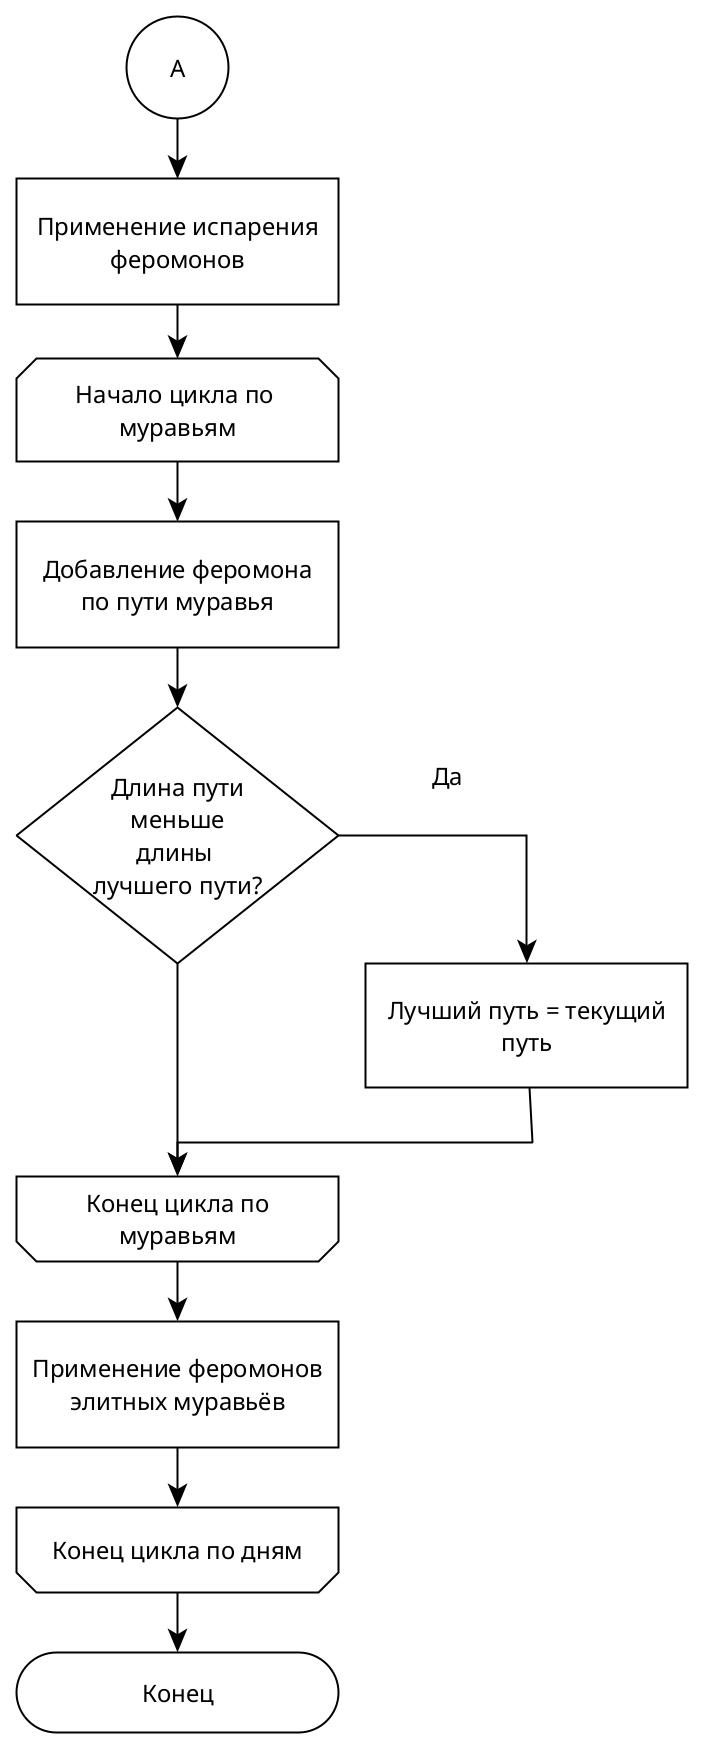
\includegraphics[width=0.5\textwidth]{ant2}
	\caption{Схема муравьиного алгоритма (конец)}
	\label{fig:ant2}
\end{figure}

\clearpage

\section{Вывод}

В результате конструкторской части были определены требования к ПО, а также разработаны схемы алгоритмов полного перебора и муравьиного алгоритма.

\clearpage
